\documentclass[border=10pt]{standalone}

\usepackage{tikz}
\usepackage{tikzsymbols}
\usetikzlibrary{calc,patterns,shapes.geometric}

\def\centerarc[#1](#2)(#3:#4:#5){\draw[#1] ($(#2)+({#5*cos(#3)},{#5*sin(#3)})$) arc (#3:#4:#5);}

\begin{document}
	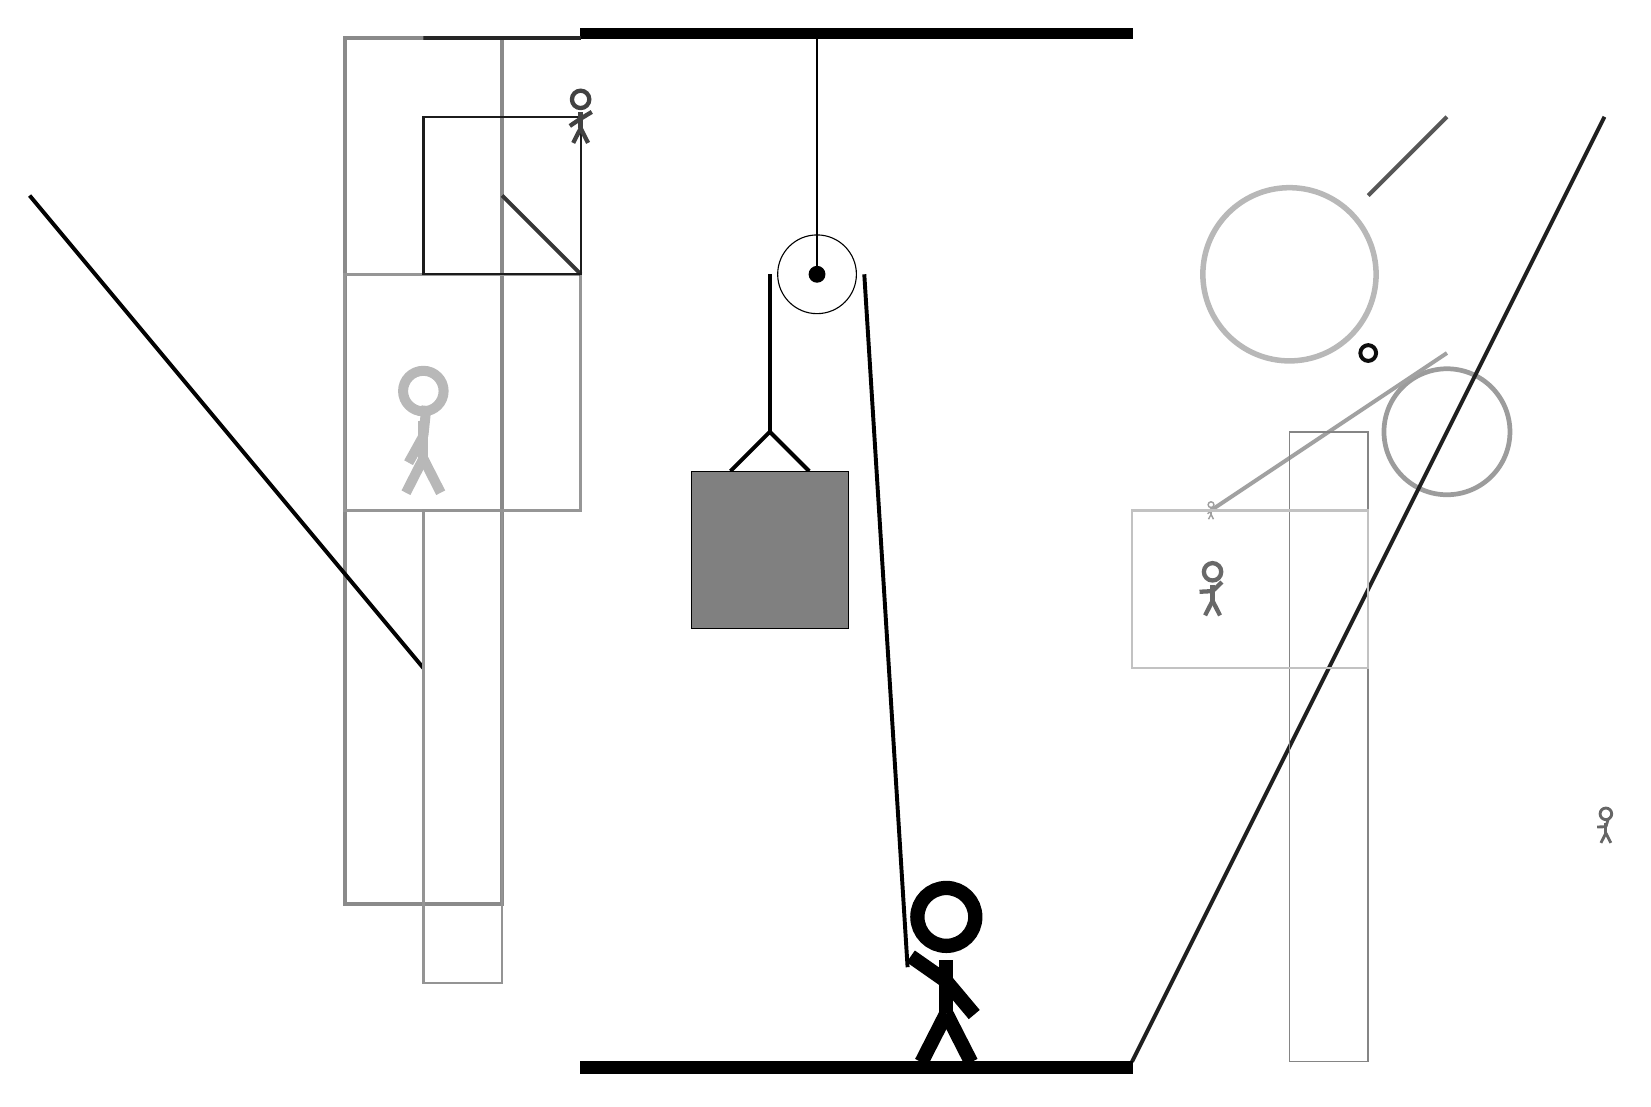
\begin{tikzpicture}
		%%%%% START %%%%%
		
		\draw[fill=black] (-2, 10) rectangle (5, 10.125);
		
		\draw (1, 7) circle (0.5);
		\draw[fill=black] (1, 7) circle (0.1);
		\draw (1, 10) -- (1, 7);
		
		\draw[line width=0.5mm] (-0.1, 4.5) -- (0.4, 5.0) -- (0.9, 4.5);
		\draw[fill=black!50] (-0.6, 4.5) rectangle (1.4, 2.5);
		
		\draw[line width=0.5mm, color=black!66](8, 8) -- (9, 9);
		
		\node[line width=0.4mm, color=black!59] at (6, 3) {\Strichmaxerl[3][3][44]};
		\draw[line width=0.5mm, color=black!46] (-3, -1) rectangle (-5, 10);
		\draw[line width=0.5mm, color=black!85] (-2, 10) rectangle (-4, 10);
		\draw[line width=0.4mm, color=black!41] (-2, 7) rectangle (-5, 4);
		\draw [line width=0.6mm, color=black!39](9, 5) circle (0.8);
		\draw[line width=0.5mm, color=black!79](-3, 8) -- (-2, 7);
		\node[line width=0.2mm, color=black!38] at (6, 4) {\Strichmaxerl[1][37][85]};
		\draw[line width=0.3mm, color=black!89] (-2, 9) rectangle (-4, 7);
		
		\node[line width=0.3mm, color=black!60] at (11, 0) {\Strichmaxerl[2][2][73]};
		\draw[line width=0.5mm, color=black!37](6, 4) -- (9, 6);
		
		\draw [line width=0.5mm, color=black!95](8, 6) circle (0.1);
		\draw[line width=0.5mm, color=black!99](-4, 2) -- (-9, 8);
		
		\draw [line width=0.7mm, color=black!28](7, 7) circle (1.1);
		\draw[line width=0.5mm, color=black!88](5, -3) -- (11, 9);
		\node[line width=0.3mm, color=black!28] at (-4, 5) {\Strichmaxerl[7][61][84]};
		\node[line width=0.7mm, color=black!74] at (-2, 9) {\Strichmaxerl[3][34][31]};
		
		\draw[line width=0.3mm, color=black!42] (-3, 4) rectangle (-4, -2);
		\draw[line width=0.2mm, color=black!48] (7, 5) rectangle (8, -3);
		\draw[line width=0.3mm, color=black!24] (5, 4) rectangle (8, 2);
		
		\draw[line width=0.5mm] (0.4, 7) -- (0.4, 5.0);
		\centerarc[line width=0.5mm](1, 7)(0:180:0.6);
		\draw[line width=0.5mm](1.6, 7) -- (2.15, -1.8);
		
		\node at (2.6, -1.9) {\Strichmaxerl[10][-35][-50]};
		
		\draw[fill=black] (-2, -3) rectangle (5, -3.15);
		
		%%%%% END %%%%%
	\end{tikzpicture}
\end{document}